\documentclass[11pt]{article}

\usepackage[margin=1in]{geometry}
\usepackage{amsmath, amssymb, amsfonts}
\usepackage{bm}
\usepackage{graphicx}
\usepackage{enumitem}
\usepackage{tikz}
\usetikzlibrary{calc}
\usepackage[most]{tcolorbox}
\usepackage{hyperref}

\title{Glacier Mass Balance Processes}
\author{Brent Minchew \\Caltech Ge 193, Spring 2026}
\date{}

\begin{document}

\maketitle

%===================================================================
% Topics Covered
%===================================================================
\section*{Topics Covered}

\begin{itemize}
  \item Mass balance definitions and terminology
  \item Accumulation and ablation processes
  \item Spatial and temporal patterns of mass balance
  \item Densification of snow to ice
  \item Ice flux and balance velocity
  \item Connecting mass balance to dynamics: continuity equation, submergence and emergence velocities, observed vs.\ balance velocity discrepancies
  \item The height--mass balance feedback and glacier response time
\end{itemize}

\bigskip
\noindent \textbf{Primary reference:} Cuffey \& Paterson, \textit{Physics of Glaciers}, 4th ed., Chapters 4 and 8.

%===================================================================
% SECTION 1 -- Introduction and Motivation
%===================================================================
\section{Introduction and Motivation}

Glaciers and ice sheets exist because snow accumulates faster than it melts in some regions of the Earth.  Over time, this snow compresses into ice under the weight of subsequent snow. The ice deforms and flows viscously under its own weight, like cold syrup spreading on a plate.  The rate at which mass is added to and removed from a glacier---the \textbf{mass balance}---is therefore the fundamental quantity linking climate to ice dynamics.  Mass balance determines the glacier's size and shape, which in turn governs the gravitational driving stress and hence how fast the ice flows.  Understanding mass balance is the essential first step toward understanding why glaciers exist, how they evolve, and how they respond to climate change.



\begin{itemize}
  \item Mass balance is the \textbf{source term} that drives ice flow.
  \item Loop (Fig. \ref{fig:4p2}):
  \begin{itemize}
  	\item Climate sets the mass balance
	\item mass balance sets the geometry
	\item geometry sets the flow
	\item flow adjusts the geometry
	\item geometry influences local to regional climate (bigger ice = bigger climate influence)
 \end{itemize}
  \item This feedback loop is the fundamental coupling between climate and glacier dynamics. 
\end{itemize}



The key question for this lecture: \textbf{How does mass balance connect to glacier dynamics?}

% Figure 4.2 (after C&P)
\begin{figure}[ht]
\centering

% --- Panel (a): Climate --> Mass Balance --> Glacier-wide Gain or Loss ---
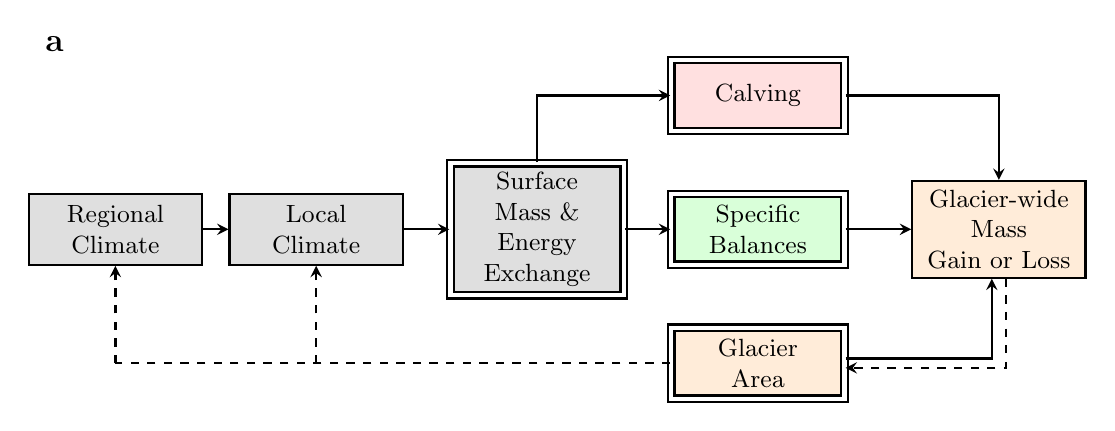
\begin{tikzpicture}[>=stealth, thick, scale=0.85,
  % Boxes only in panel (a): solid border
  graybox/.style={draw, fill=gray!25, minimum width=2.2cm, minimum height=0.9cm,
                  align=center, font=\small},
  orangebox/.style={draw, fill=orange!15, minimum width=2.2cm, minimum height=0.9cm,
                    align=center, font=\small},
  % Boxes shared between panels: double border
  greenbox/.style={draw, double, double distance=1.5pt, fill=green!15,
                   minimum width=2.2cm, minimum height=0.9cm, align=center, font=\small},
  redbox/.style={draw, double, double distance=1.5pt, fill=red!12,
                 minimum width=2.2cm, minimum height=0.9cm, align=center, font=\small},
  orangebox_shared/.style={draw, double, double distance=1.5pt, fill=orange!15,
                           minimum width=2.2cm, minimum height=0.9cm, align=center, font=\small},
  graybox_shared/.style={draw, double, double distance=1.5pt, fill=gray!25,
                         minimum width=2.2cm, minimum height=0.9cm, align=center, font=\small}
]
  % Panel label
  \node[anchor=south west, font=\bfseries\large] at (-1.2,2.5) {a};

  % Main row
  \node[graybox] (regional) at (0,0) {Regional\\Climate};
  \node[graybox] (local) at (3,0) {Local\\Climate};
  \node[graybox_shared] (exchange) at (6.3,0) {Surface\\Mass \&\\Energy\\Exchange};
  \node[greenbox] (specific) at (9.6,0) {Specific\\Balances};
  \node[orangebox] (gainloss) at (13.2,0) {Glacier-wide\\Mass\\Gain or Loss};

  % Calving (above)
  \node[redbox] (calving) at (9.6,2) {Calving};

  % Glacier Area (below)
  \node[orangebox_shared] (area) at (9.6,-2) {Glacier\\Area};

  % Solid arrows along main chain
  \draw[->] (regional) -- (local);
  \draw[->] (local) -- (exchange);
  \draw[->] (exchange) -- (specific);
  \draw[->] (specific) -- (gainloss);

  % Solid arrow: Surface Mass & Energy Exchange to Calving
  \draw[->] (exchange.north) |- (calving.west);

  % Calving arrow into Glacier-wide Mass Gain or Loss
  \draw[->] (calving.east) -| (gainloss.north);

  % Solid arrow: Glacier Area to Glacier-wide Mass Gain or Loss
  \draw[->] ([yshift=2pt]area.east) -| ([xshift=-3pt]gainloss.south);

  % Dashed feedback: Glacier-wide Mass Gain or Loss to Glacier Area
  \draw[->, dashed] ([xshift=3pt]gainloss.south) |- ([yshift=-2pt]area.east);

  % Dashed feedback: Glacier Area to Regional Climate (horizontal, right turn up)
  % with a vertical dashed arrow branching up to Local Climate
  \draw[dashed] (area.west) -- (regional.south |- area)
    coordinate (feedback_turn);
  \draw[->, dashed] (feedback_turn) -- (regional.south);
  \draw[->, dashed] (local.south |- feedback_turn) -- (local.south);

\end{tikzpicture}

\vspace{1.2cm}

% --- Panel (b): Dynamics feedback loop ---
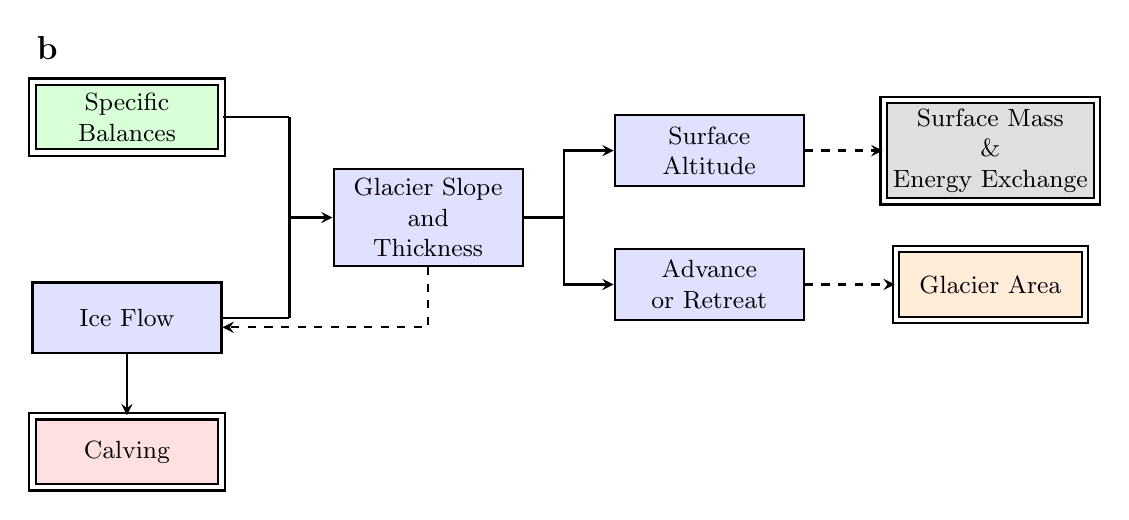
\begin{tikzpicture}[>=stealth, thick, scale=0.85,
  % Boxes only in panel (b): solid border
  bluebox/.style={draw, fill=blue!12, minimum width=2.4cm, minimum height=0.9cm,
                  align=center, font=\small},
  % Boxes shared between panels: double border
  greenbox/.style={draw, double, double distance=1.5pt, fill=green!15,
                   minimum width=2.4cm, minimum height=0.9cm, align=center, font=\small},
  redbox/.style={draw, double, double distance=1.5pt, fill=red!12,
                 minimum width=2.4cm, minimum height=0.9cm, align=center, font=\small},
  orangebox_shared/.style={draw, double, double distance=1.5pt, fill=orange!15,
                           minimum width=2.4cm, minimum height=0.9cm, align=center, font=\small},
  graybox_shared/.style={draw, double, double distance=1.5pt, fill=gray!25,
                         minimum width=2.4cm, minimum height=0.9cm, align=center, font=\small}
]
  % Panel label
  \node[anchor=south west, font=\bfseries\large] at (-1.5,2.2) {b};

  % Left column
  \node[greenbox] (specific) at (0,1.5) {Specific\\Balances};
  \node[bluebox]  (iceflow)  at (0,-1.5) {Ice Flow};
  \node[redbox]   (calving)  at (0,-3.5) {Calving};

  % Center column
  \node[bluebox] (slope) at (4.5,0) {Glacier Slope\\and\\Thickness};

  % Right branches
  \node[bluebox] (altitude) at (8.7,1.0) {Surface\\Altitude};
  \node[bluebox] (advance)  at (8.7,-1.0) {Advance\\or Retreat};

  % Far right (minimized gap)
  \node[graybox_shared] (surfexch) at (12.9,1.0) {Surface Mass\\\&\\Energy Exchange};
  \node[orangebox_shared] (glacarea) at (12.9,-1.0) {Glacier Area};

  % --- Solid arrows: Specific Balances & Ice Flow into Glacier Slope and Thickness ---
  % Horizontal lines from each box
  \draw (specific.east) -- ++(1.0,0) coordinate (sp_end);
  \draw (iceflow.east)  -- ++(1.0,0) coordinate (if_end);
  % Vertical line joining them
  \draw (sp_end) -- (if_end);
  % Arrow from midpoint of vertical line into Glacier Slope and Thickness
  \coordinate (mid_join) at ($(sp_end)!0.5!(if_end)$);
  \draw[->] (mid_join) -- (slope.west);

  % Solid arrow: Ice Flow to Calving
  \draw[->] (iceflow) -- (calving);

  % Dashed feedback: Glacier Slope and Thickness to Ice Flow (small vertical offset)
  \coordinate (if_offset) at ($(iceflow.east)+(0,-4pt)$);
  \draw[->, dashed] (slope.south) -- (slope.south |- if_offset) -- (if_offset);

  % Solid arrows: Glacier Slope --> Surface Altitude, Glacier Slope --> Advance or Retreat
  \draw[->] (slope.east) -- ++(0.6,0) coordinate (branch) |- (altitude.west);
  \draw[->] (branch) |- (advance.west);

  % Dashed arrows: Surface Altitude --> Surface Mass & Energy Exchange
  \draw[->, dashed] (altitude) -- (surfexch);

  % Dashed arrows: Advance or Retreat --> Glacier Area
  \draw[->, dashed] (advance) -- (glacarea);

\end{tikzpicture}

\caption{After Fig.~4.2 in C\&P.  Generalized factors determining the relation between climate, ice flow, and glacier mass balance.  Feedbacks are indicated by dashed lines.  The chart has been separated into two parts for clarity (panels \textbf{a} and \textbf{b}).  Double-bordered boxes appear in both panels.  Colors indicate role: gray = climate forcing, green = mass balance (the bridge between climate and dynamics), blue = glacier dynamics, orange = observable state/outcomes, pink = calving (mass-loss pathway).}
\label{fig:4p2}
\end{figure}

%===================================================================
% SECTION 2 -- Definitions and Terminology
%===================================================================
\section{Definitions and Terminology}

\subsection{Specific Balance Rate}

The \textbf{specific balance} represents the change of mass per unit area at a point on the glacier.  The specific balance rate $\dot{b}$ has units of kg\,m$^{-2}$\,yr$^{-1}$.

For ice dynamics, the most useful form is the \textbf{ice-equivalent rate}:
\begin{equation}
  \dot{b}_i = \frac{\dot{b}}{\rho_i} \quad (\text{m\,yr}^{-1}),
\end{equation}
where $\rho_i$ is the mass density of ice ($800\le\rho_i\le917$ kg/m$^3$).

Field studies commonly report \textbf{water-equivalent rates}:
\begin{equation}
  \dot{b}_w = \frac{\dot{b}}{\rho_w} = \frac{\rho_i}{\rho_w}\,\dot{b}_i \quad (\text{m\,w.eq.\,yr}^{-1}).
  \tag{C\&P Eq.~4.1}
\end{equation}

\subsection{Components of the Specific Balance}

The specific balance can be subdivided according to where the mass exchange occurs along a vertical column:
\begin{equation}
  \dot{b} = \dot{b}_s + \dot{b}_e + \dot{b}_b,
\end{equation}
where $\dot{b}_s$ is the surface balance, $\dot{b}_e$ the englacial balance, and $\dot{b}_b$ the basal balance.

In most cases, the surface balance dominates: $\dot{b} \approx \dot{b}_s$.  Basal balance can be important for floating ice shelves and glaciers on volcanoes.  For Antarctic ice shelves, basal melting by the ocean actually exceeds iceberg calving as a mass-loss mechanism, with continent-wide estimates of $\sim$1300--1500~Gt\,yr$^{-1}$ (Rignot et al., 2013; Adusumilli et al., 2020).

\subsection{Accumulation and Ablation}

\textbf{Accumulation} refers to all processes by which snow and ice are added to a glacier.  

\noindent\textbf{Ablation} refers to all processes of removal.

The surface balance rate at a point is:
\begin{equation}
  \dot{b}_s = \dot{a}_s + \dot{a}_a - \dot{m}_s + \dot{a}_r - \dot{s} + \dot{a}_w,
  \tag{C\&P Eq.~4.3}
\end{equation}
representing snowfall ($\dot{a}_s$), avalanche deposition ($\dot{a}_a$), melt ($\dot{m}_s$), refreezing of water ($\dot{a}_r$), sublimation ($\dot{s}$), and wind deposition ($\dot{a}_w$).

On most glaciers, snowfall and melt dominate:
\begin{equation}
  \dot{b}_s \approx \dot{a}_s - \dot{m}_s.
\end{equation}

\subsection{Whole-Glacier Balance}

The total rate of mass change of a glacier with plan-view area $\mathcal{A}$ is:
\begin{equation}
  \frac{dM}{dt} = \int_{\mathcal{A}} \left[\dot{b}_s + \dot{b}_e + \dot{b}_b\right] d\mathcal{A} - \dot{B}_c,
  \tag{C\&P Eq.~4.2}
\end{equation}
where $\dot{B}_c$ is the mass per unit time lost by calving.

The annual glacier balance $B_n$ and average specific balance are:
\begin{equation}
  B_n = \int_{\mathcal{A}} b_n \, d\mathcal{A} \qquad \text{and} \qquad \bar{b}_n = \frac{B_n}{\mathcal{A}}.
  \tag{C\&P Eq.~4.7}
\end{equation}

%===================================================================
% SECTION 3 -- Spatial and Temporal Patterns
%===================================================================
\section{Spatial and Temporal Patterns}

\subsection{The Seasonal Cycle}

The surface balance rate varies over the year: In general, accumulation dominates in winter and ablation in summer. Most of Antarctica only accumulates; ablation is through glacier flow.

% CHALKBOARD DRAWING 2:
% Sketch the seasonal cycle (Fig. 4.3 in C&P).
% Time on x-axis, specific mass change on y-axis.
% Draw accumulation curve rising through winter, then ablation pulling it down in summer.
% Mark: end-of-winter max, end-of-summer min, winter balance, summer balance, annual (net) balance.
% Label t_1, t_m, t_2 (balance year boundaries).

Key definitions:
\begin{itemize}
  \item \textbf{Balance year:} the interval between two successive mass minima (typically $\sim$365 days).
  \item \textbf{Winter balance:} mass gained during the winter season ($t_1$ to $t_m$).
  \item \textbf{Summer balance:} mass lost during the summer season ($t_m$ to $t_2$).
  \item \textbf{Annual (net) balance} $b_n$: specific balance at the end of the balance year.
\end{itemize}

\subsection{Variation with Altitude}

% CHALKBOARD DRAWING 3:
% (a) Draw the classic "balance vs. altitude" plot (Fig. 4.5a style).
%     Vertical axis = elevation, horizontal axis = annual balance (m).
%     Curve crosses zero at the ELA.  Label accumulation zone above, ablation zone below.
% (b) On a separate sketch, draw the glacier in side-view cross-section.
%     Mark the ELA, annotate where b > 0 and b < 0, and draw arrows showing flow direction.

The specific balance varies strongly with altitude:
\begin{itemize}
  \item \textbf{Accumulation zone} ($b_n > 0$): broad upper region of mass surplus.
  \item \textbf{Ablation zone} ($b_n < 0$): lower region of mass deficit.
  \item \textbf{Equilibrium Line Altitude (ELA):} the altitude where $b_n = 0$.
  \item \textbf{Accumulation Area Ratio (AAR):} ratio of accumulation-zone area to total glacier area; typically $\sim$0.5--0.7 for glaciers near balance.
\end{itemize}

The \textbf{mass balance gradient} $db_n/dz$ reflects climate setting:
\begin{itemize}
  \item Temperate (aka maritime) glaciers (e.g., Nigardsbreen, Norway): large gradient, large mass turnover.
  \item Continental/polar glaciers (e.g., White Glacier, Arctic Canada): small gradient, small mass turnover.
\end{itemize}

\subsection{Relation to Temperature and Precipitation}

Temperature is the dominant control on elevation gradients of surface balance:
\begin{enumerate}
  \item In cold climates ($\bar{T} \lesssim -15\,^{\circ}$C): almost no melt; balance controlled by precipitation (Clausius--Clapeyron relation governs saturation vapor pressure, so snowfall increases exponentially with temperature).
  \item In warm climates: balance controlled mainly by melt, which increases sharply with temperature.
\end{enumerate}

This explains why temperate (maritime) glaciers have large mass turnovers and continental glaciers have small turnovers.

%===================================================================
% SECTION 4 -- Densification of Snow to Ice
%===================================================================
\section{Densification of Snow to Ice}

Snow that accumulates on a glacier surface is progressively transformed into glacier ice through a process called \textbf{densification} (or firnification).  Understanding this process matters because (1) it determines how surface accumulation translates into ice volume, and (2) it controls the density structure of the upper glacier, which affects remote sensing observations and mass balance estimates.

\subsection{Stages of Densification}

Fresh snow has a density of roughly $50$--$200$~kg\,m$^{-3}$, whereas glacier ice has a density of $\rho_i \approx 917$~kg\,m$^{-3}$.  The transformation proceeds through three stages:

\begin{enumerate}
  \item \textbf{Snow to firn} ($\rho \lesssim 550$~kg\,m$^{-3}$): Settling, rounding of snow grains, and mechanical packing dominate.  Wind and surface melt--refreeze cycles accelerate the process.  Snow is reclassified as \textbf{firn} (granular, multi-year snow that has survived at least one melt season) once it has densified beyond fresh snow.

  \item \textbf{Firn densification} ($550 \lesssim \rho \lesssim 830$~kg\,m$^{-3}$): Sintering and plastic deformation of ice grains become the primary mechanisms as overburden pressure increases with depth.  Air passages between grains remain connected, so the material is still permeable.

  \item \textbf{Pore close-off and bubble trapping} ($\rho \approx 830$~kg\,m$^{-3}$): Air passages pinch shut, trapping bubbles within the ice matrix.  Below this density, further compression of the trapped bubbles slowly increases density toward $917$~kg\,m$^{-3}$.  The depth at which pore close-off occurs is called the \textbf{firn--ice transition}.
\end{enumerate}

% CHALKBOARD DRAWING:
% Sketch a density--depth profile (density on x-axis, depth on y-axis increasing downward).
% Mark the three stages: rapid densification near the surface, slower densification through the firn column,
% and the pore close-off density (~830 kg/m^3).  Label the firn--ice transition depth.

\subsection{Controls on Densification Rate}

The rate at which firn densifies depends on:
\begin{itemize}
  \item \textbf{Accumulation rate:} Higher accumulation buries snow more quickly, increasing overburden pressure at a given age but also meaning that a given depth corresponds to younger (less densified) material.  The net effect is that high-accumulation sites tend to have \emph{deeper} firn columns.
  \item \textbf{Temperature:} Warmer firn densifies faster because ice creep rates increase with temperature.  On temperate glaciers, meltwater percolation and refreezing dramatically accelerate densification, producing thin firn layers or even eliminating the firn column entirely.
  \item \textbf{Grain size and impurities:} Smaller grains sinter more readily; impurities can inhibit or promote grain-boundary processes.
\end{itemize}

Firn column thickness ranges from zero on temperate glaciers (where surface melt removes or compacts the firn) to $\sim$60--120~m in the cold, dry interior of Antarctica and Greenland.

\subsection{Implications for Mass Balance and Ice Dynamics}

\begin{itemize}
  \item \textbf{Column-average density:} When converting between ice-equivalent thickness and actual thickness, the density profile through the firn must be accounted for.  The column-average density $\bar{\rho}$ appearing in flux calculations is less than $\rho_i$ wherever a significant firn layer exists.
  \item \textbf{Firn compaction vs.\ mass change:} Surface elevation changes measured by altimetry reflect both mass changes and firn compaction.  Densification models are needed to separate the two contributions---a major source of uncertainty in ice-sheet mass balance estimates from satellite altimetry.
  \item \textbf{Meltwater storage:} The pore space in firn can store meltwater, buffering runoff.  This firn aquifer effect has been observed in southeastern Greenland, where meltwater persists year-round within the firn column.
\end{itemize}

%===================================================================
% SECTION 5 -- From Mass Balance to Ice Flux
%===================================================================
\section{From Mass Balance to Ice Flux}

\subsection{Ice Flux}

The volumetric ice flux per unit width through a cross-section is:
\begin{equation}
  q = \int_{bed}^{surface}u(z)dz = \bar{u}h,
\end{equation}
where $\bar{u}$ is the depth-averaged horizontal velocity and $h$ is the ice thickness.

Mass flux through a cross-section is $Q = \int_{bed}^{surface} \rho(z)\, u(z) \, dz$.

Measured fluxes span several orders of magnitude (Table 8.1 in C\&P): from small mountain glaciers ($q \sim 0.3 \times 10^4$ m$^2$\,yr$^{-1}$) to major ice-sheet outlets like Sermeq Kujalleq (Jakobshavn Isbr\ae), Greenland ($q \sim 670 \times 10^4$ m$^2$\,yr$^{-1}$).

\subsection{What Determines the Flux?}

Two approaches:
\begin{enumerate}
  \item \textbf{Mechanical approach:} force balance $\to$ flow law $\to$ velocity $\to$ flux.  Always valid, but uncertainties in basal conditions often limit predictive power.
  \item \textbf{Mass conservation approach:} if the glacier is near steady state, the flux is determined by the upstream accumulation.
\end{enumerate}

The second approach leads directly to the concept of \textbf{balance velocity}.

%===================================================================
% SECTION 5 -- Derivation of Balance Velocity (centerpiece)
%===================================================================
\section{Balance Velocity}

\subsection{Starting Premise: Steady State}

If the glacier is not changing significantly over a period of years, $dM/dt \approx 0$.  Even when glaciers are changing, the rate of mass gain or loss is often small compared to the total flux, provided we average over several years (smoothing out short-term variability in snowfall and melt).

Setting $dM/dt = 0$ gives an approximation for the rate of flow based on the equality of inputs and outflow.

% CHALKBOARD DRAWING 4:
% Draw Figure 8.1 from the textbook:
% Plan view of a glacier.  At some distance X from the head, draw a cross-section
% ("flux gate") of width Y and thickness h.
% Shade the upstream drainage area A = X * W (W = average width upstream).
% Show arrows for flow direction and the flux gate.

\subsection{The Mass Balance Integral}

All ice accumulated over the upstream drainage area $\mathcal{A}$ must pass through the cross-section.  Setting input equal to output:
\begin{equation}
  \boxed{
  \rho_i \int_{\mathcal{A}} \dot{b}_i \, d\mathcal{A} = \bar{\rho}\, h\, U_B\, Y
  }
  \tag{C\&P Eq.~8.3}
\end{equation}
where:
\begin{itemize}
  \item $\dot{b}_i$ is the specific mass balance rate (ice equivalent, m\,yr$^{-1}$), varying over the upstream area $\mathcal{A}$
  \item $h$ is the ice thickness at the cross-section
  \item $Y$ is the width of the glacier at the cross-section
  \item $U_B$ is the \textbf{balance velocity} (depth-averaged)
  \item $\bar{\rho}$ is the column-average density ($\approx \rho_i$ below the firn layer)
\end{itemize}

% CHALKBOARD DRAWING 5 (key derivation figure):
% Re-draw the glacier from above.  Label the upstream area A, the cross-section with h and Y.
% Write "mass in" = b-dot * A on one side and "mass out" = U_B * h * Y on the other.
% Draw an equals sign between them, then rearrange to isolate U_B.  Box the final result.

\subsection{Solving for the Balance Velocity}

Taking $\bar{\rho} \approx \rho_i$ and solving for $U_B$:
\begin{equation}
  \boxed{
  U_B = \frac{1}{h\,Y} \int_{\mathcal{A}} \dot{b}_i \, d\mathcal{A}
  }
\end{equation}

If we define $\overline{\dot{b}}_i$ as the area-averaged specific balance over the basin area $\mathcal{A} = X\,W$ (where $X$ is the distance from the head and $W$ is the mean upstream width), this simplifies to:
\begin{equation}
  U_B = \frac{\overline{\dot{b}}_i\, X\, W}{h\, Y}.
\end{equation}

\subsection{Physical Interpretation}

The balance velocity increases with:
\begin{enumerate}
  \item \textbf{Larger upstream area} ($\mathcal{A} = XW$): more accumulation to evacuate $\Rightarrow$ higher $U_B$.
  \item \textbf{Larger specific balance} ($\dot{b}_i$): more mass input $\Rightarrow$ higher $U_B$.
\end{enumerate}

The balance velocity decreases with:
\begin{enumerate}[resume]
  \item \textbf{Thicker ice} ($h$): taller conduit for flux $\Rightarrow$ lower $U_B$ needed.
  \item \textbf{Wider glacier} ($Y$): wider conduit $\Rightarrow$ lower $U_B$ needed.
\end{enumerate}

% CHALKBOARD DRAWING 6:
% Draw a side-view longitudinal profile of a glacier (elevation vs. distance along flowline).
% Below it, sketch U_B vs. distance.
% U_B = 0 at the head, rises to a maximum near the ELA, decreases toward the terminus
% (reaching zero at the snout for a land-terminating glacier).
% Annotate: "maximum flux ~ ELA", "accumulation zone", "ablation zone".

\medskip
\noindent \textbf{Key result:} $U_B$ is zero at the glacier head, increases to a maximum near the ELA (where cumulative accumulation is largest relative to $hY$), and decreases toward the terminus as ablation removes mass from the upstream area.

In a steady state, the annual flux through a cross-section in the accumulation zone must equal the total annual accumulation upstream.  In the ablation zone, the flux must equal the mass of ice lost by ablation between the cross-section and the terminus.  Thus, the flux increases from the head to the equilibrium line and decreases from there to the terminus.

\subsection{Computing Balance Velocities in Practice}

To construct a balance velocity map (e.g., Figs.~8.2a,b in C\&P for Greenland and Antarctica), one needs:
\begin{itemize}
  \item \textbf{Surface topography} (to determine flow direction and delineate drainage basins, assuming flow is perpendicular to surface elevation contours).
  \item \textbf{Ice thickness} $h$ (from ice-penetrating radar).
  \item \textbf{Specific balance} $\dot{b}_i$ (from climate models, reanalysis, or field observations).
\end{itemize}

Balance velocities provide a useful estimate of flow fields even in remote areas, and have been computed for both ice sheets.  The maps reveal the concentration of flow into narrow, fast-flowing ice streams and outlet glaciers near the margins.

\begin{figure}[ht]
  \centering
  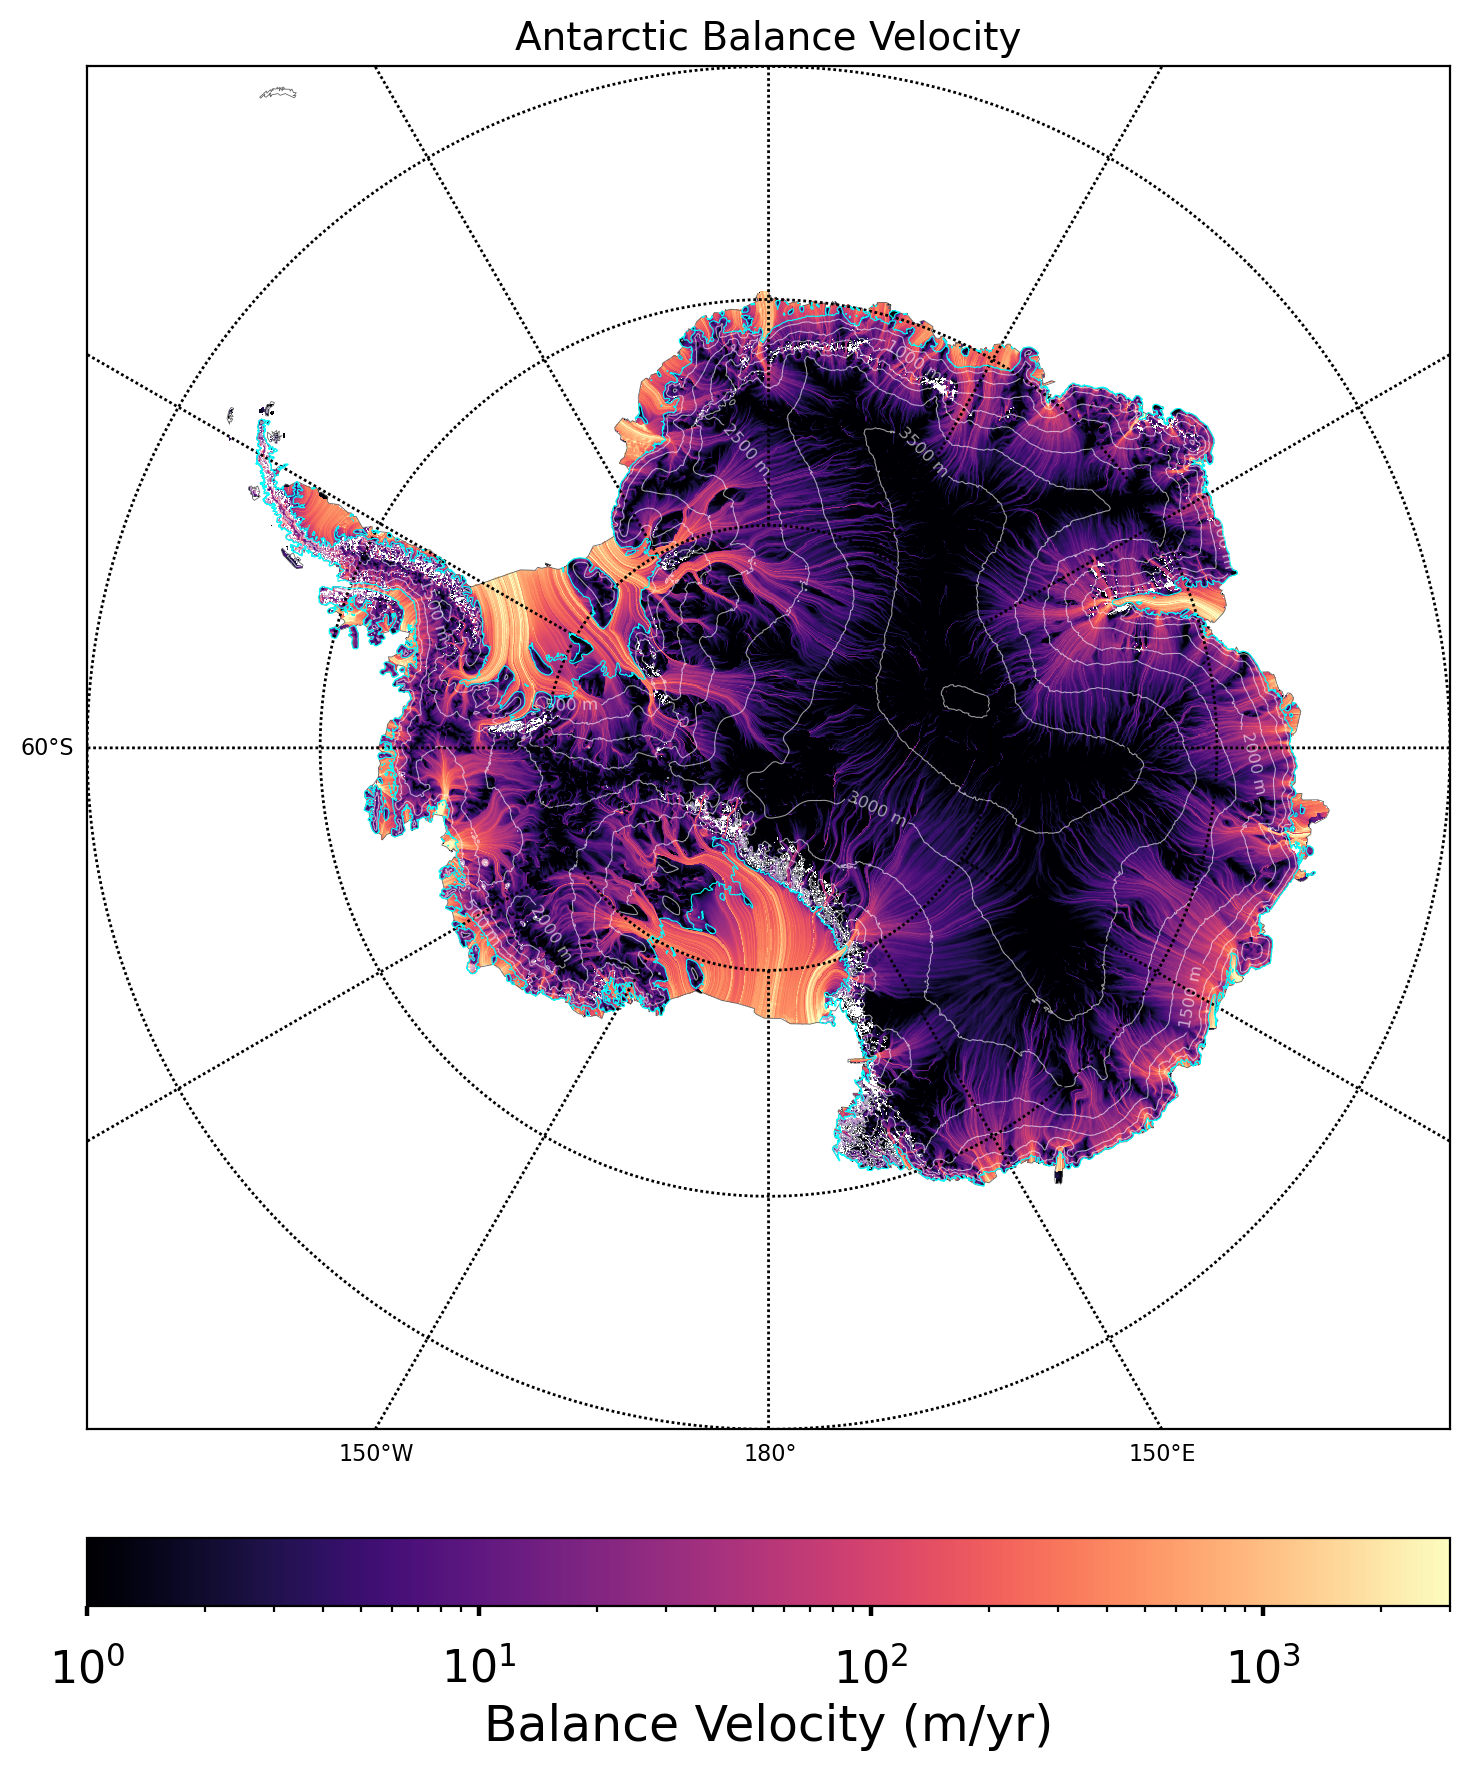
\includegraphics[width=0.48\textwidth]{figures/BalanceVelocity_map.png}
  \hfill
  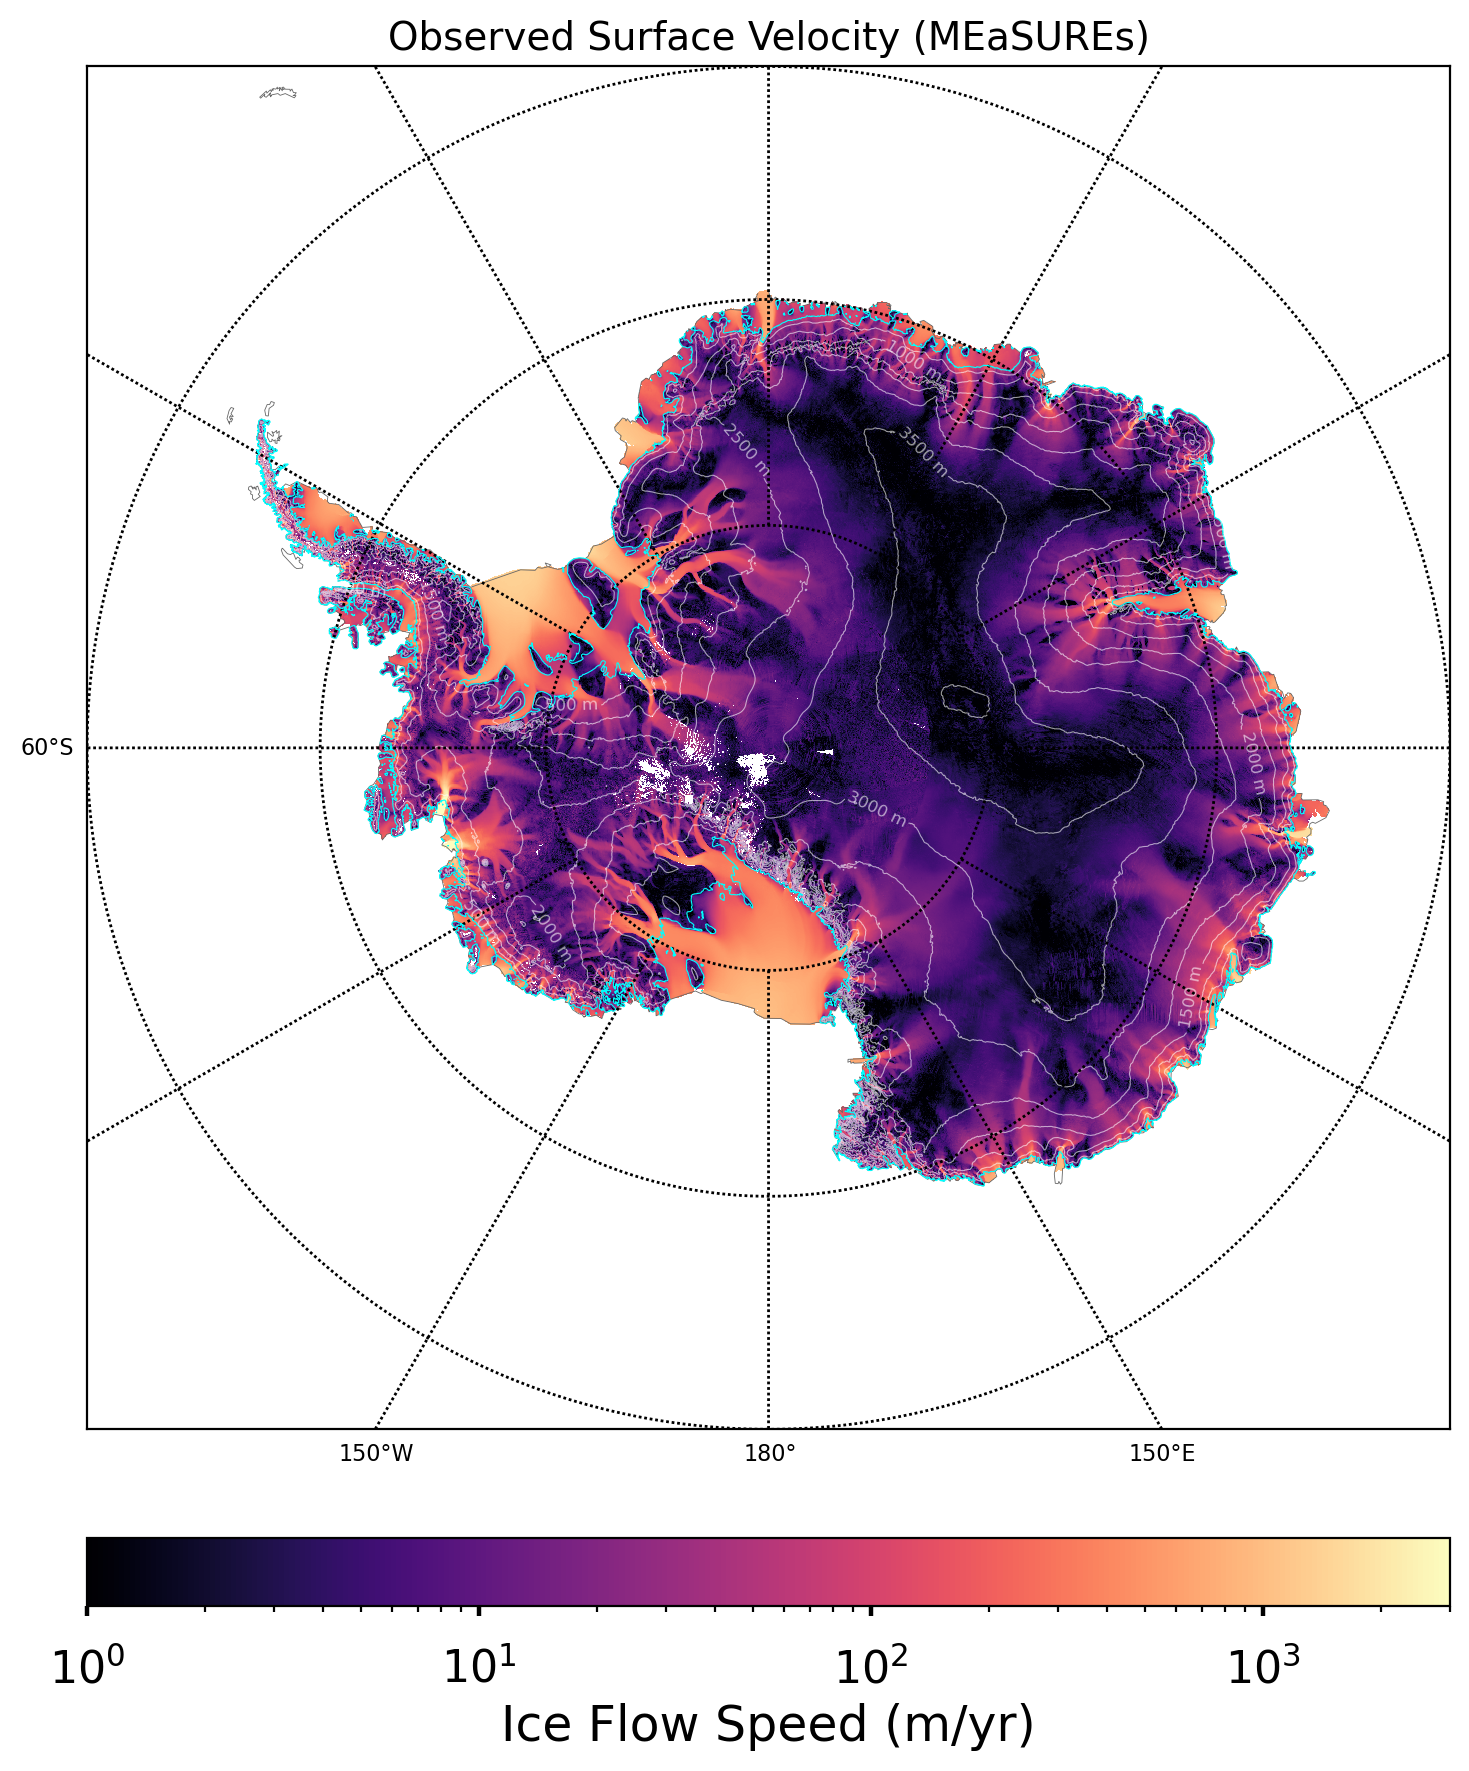
\includegraphics[width=0.48\textwidth]{figures/ObservedVelocity_map.png}
  \caption{Balance velocity (left) and observed velocity (right).}
  \label{fig:balance_observed_velocity}
\end{figure}

%\begin{figure}[ht]
 % \centering
 % 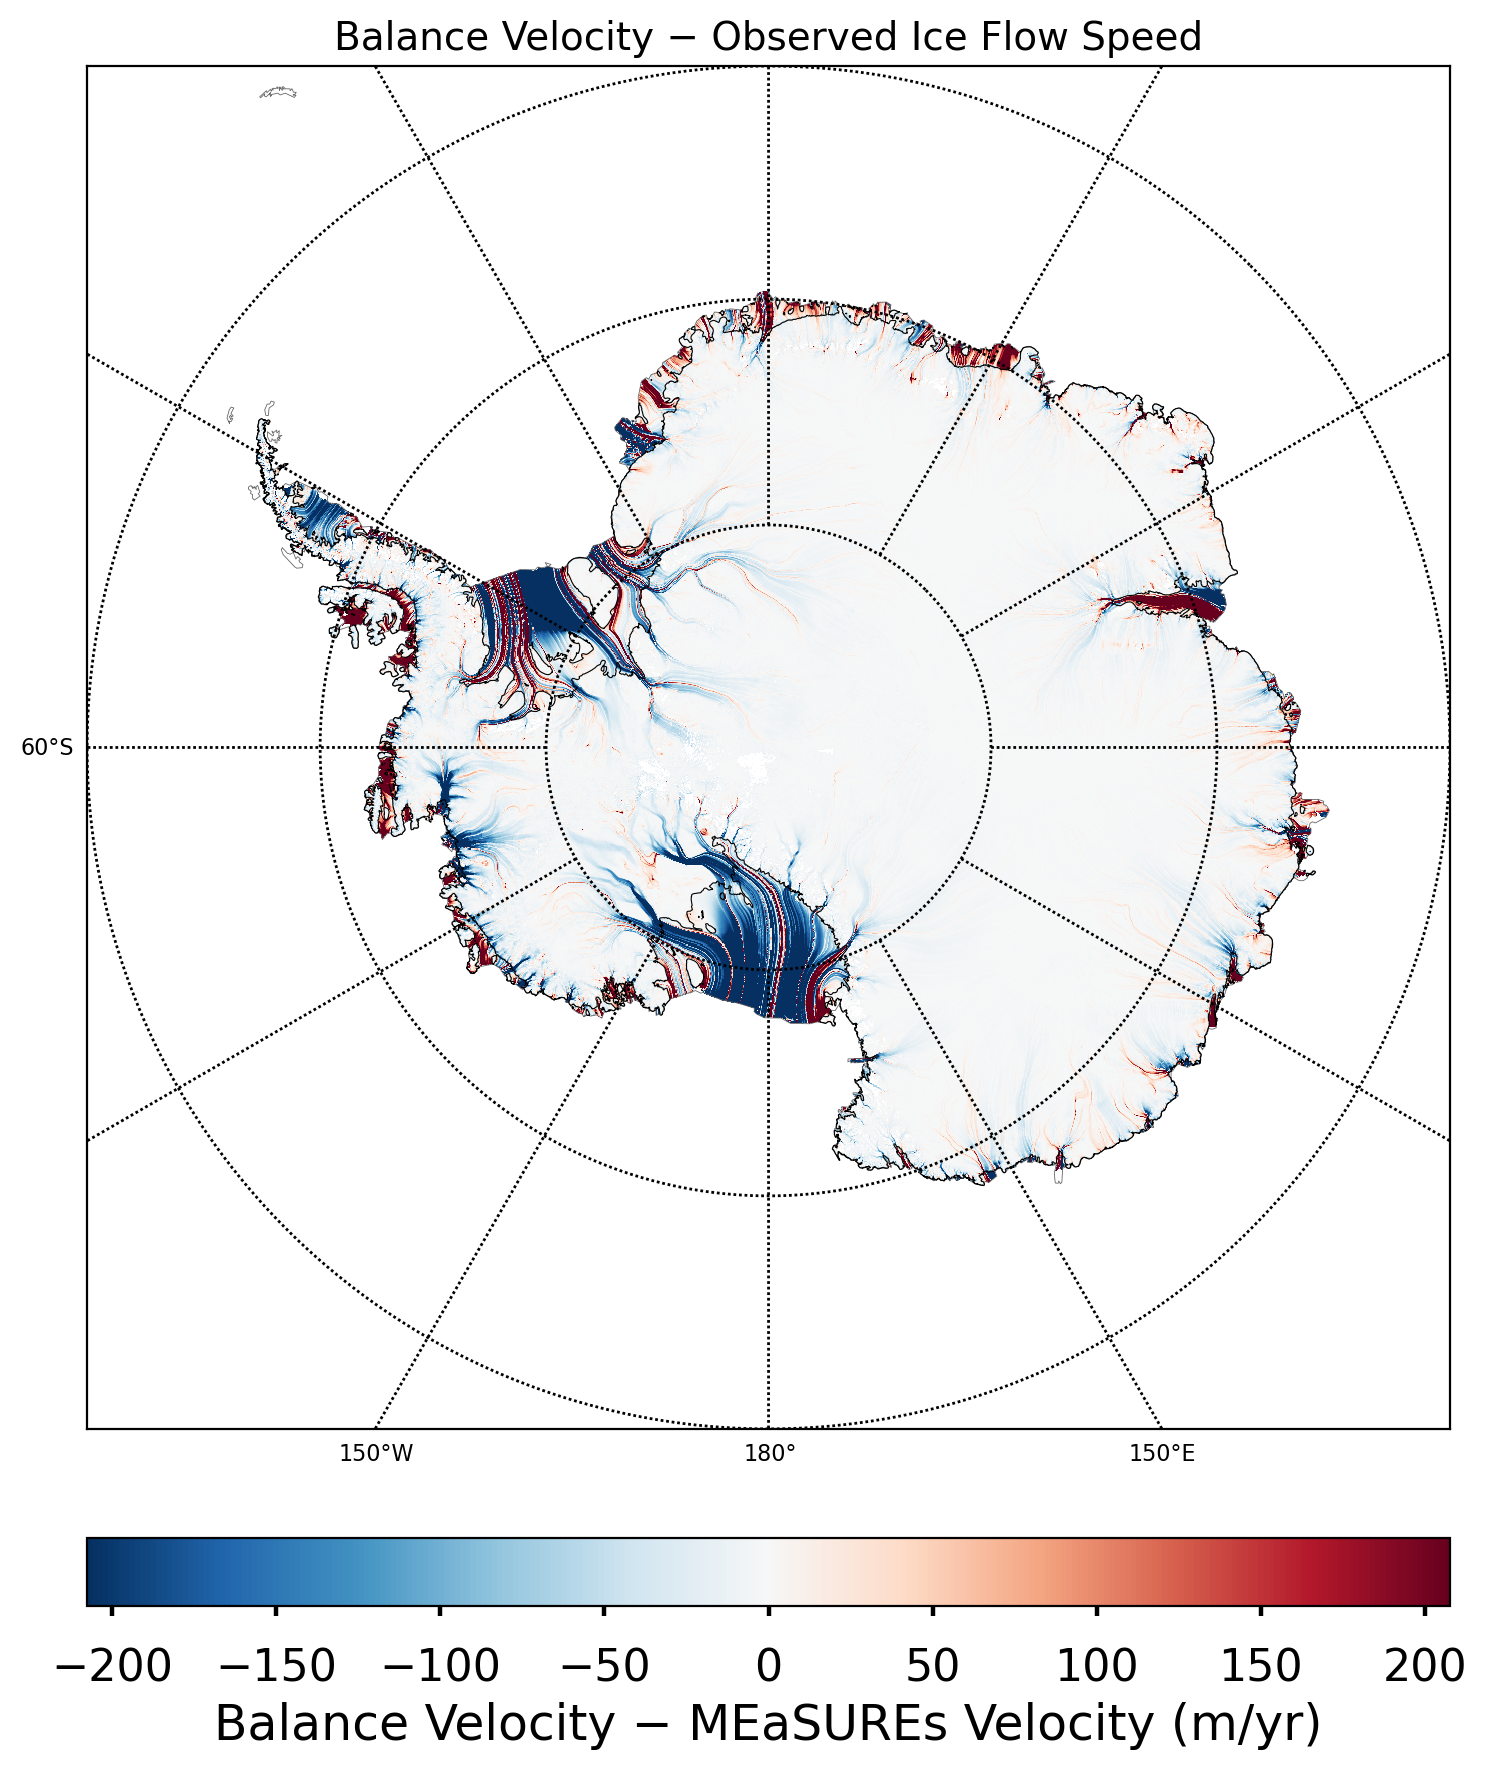
\includegraphics[width=0.6\textwidth]{figures/BalanceVelocity_difference.png}
 % \caption{Difference between balance velocity and observed velocity.}
  %\label{fig:balance_velocity_difference}
%\end{figure}

%===================================================================
% SECTION 7 -- Connecting to Dynamics
%===================================================================
\section{Connecting to Dynamics: Balance vs.\ Actual Velocity}

\subsection{The Vertically Integrated Continuity Equation}

The balance velocity derivation is a special case of the more general mass conservation relation, aka the continuity equation and kinematic boundary condition. These terms all refer to the same equation, with the general form in two horizontal dimensions:
\begin{equation}
  \frac{\partial h}{\partial t} = \dot{b}_i - \bm{\nabla} \cdot \bm{q},
  \tag{C\&P Eq.~8.79}
\end{equation}
where $\bm{q} = \bar{u}\,h$ is the depth-integrated volume flux vector.

% CHALKBOARD DRAWING 7:
% Draw the schematic of a vertical ice column (Fig. 8.16 in C&P).
% Show b-dot_s entering from the top, b-dot_b at the base,
% horizontal flux Q entering one side and Q + dQ leaving the other.
% Write the continuity equation as: "what comes in must go out, or the column thickness changes."

\medskip
\noindent At steady state ($\partial h/\partial t = 0$):
\begin{equation}
  \dot{b}_i = \bm{\nabla} \cdot \bm{q}.
\end{equation}
The balance velocity condition is the integrated form of this relation.



\begin{tcolorbox}[
  colback=orange!25,
  colframe=orange!70!black,
  title={\textbf{Derivation: The Vertically Integrated Continuity Equation}},
  fonttitle=\bfseries,
  breakable
]

Consider a column of ice between positions $x$ and $x + \delta x$, with thickness $h(x,t)$ and unit width into the page.  Mass balance $\dot{b}_i$ adds or removes ice at the surface.

\medskip
\begin{center}
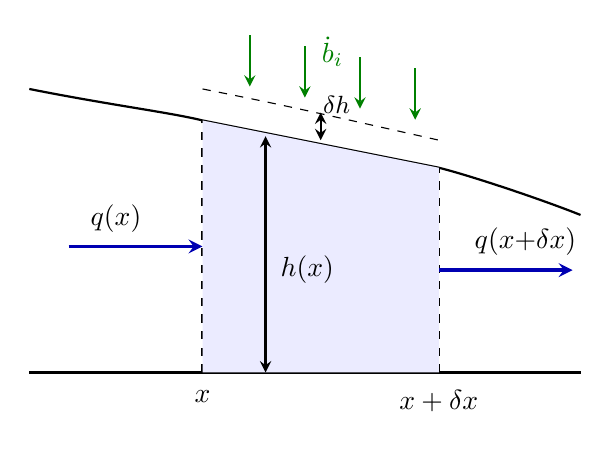
\begin{tikzpicture}[>=stealth, thick]
  % Bed
  \draw[very thick] (0,0) -- (7,0);
  \node[below] at (2.2,-0.1) {$x$};
  \node[below] at (5.2,-0.1) {$x + \delta x$};

  % Dashed verticals for the column
  \draw[dashed] (2.2,0) -- (2.2,3.2);
  \draw[dashed] (5.2,0) -- (5.2,2.6);

  % Ice surface (sloping)
  \draw[thick] (0,3.6) .. controls (1,3.4) and (1.8,3.3) .. (2.2,3.2)
    -- (5.2,2.6) .. controls (5.6,2.5) and (6.5,2.2) .. (7,2.0);

  % Dashed surface showing change delta h
  \draw[dashed, thin] (2.2,3.6) .. controls (3.2,3.4) .. (5.2,2.95);
  \draw[<->] (3.7,3.3) -- (3.7,2.95);
  \node[right] at (3.6,3.4) {\small $\delta h$};

  % Flux arrow in (left)
  \draw[->, very thick, blue!70!black] (0.5,1.6) -- (2.2,1.6);
  \node[above] at (1.1,1.65) {$q(x)$};

  % Flux arrow out (right)
  \draw[->, very thick, blue!70!black] (5.2,1.3) -- (6.9,1.3);
  \node[above] at (6.3,1.35) {$q(x{+}\delta x)$};

  % Mass balance arrows (top, into column)
  \foreach \xpos in {2.8, 3.5, 4.2, 4.9} {
    \draw[->, green!50!black] (\xpos, {3.6 - (\xpos-2.2)*0.2 + 0.8})
      -- (\xpos, {3.6 - (\xpos-2.2)*0.2 + 0.15});
  }
  \node[above, green!50!black] at (3.85, 3.75) {$\dot{b}_i$};

  % Ice fill (light)
  \fill[blue!8] (2.2,0) -- (2.2,3.2) -- (5.2,2.6) -- (5.2,0) -- cycle;

  % Thickness label
  \draw[<->] (3,0) -- (3,3);
  \node[left] at (4,1.3) {$h(x)$};
\end{tikzpicture}
\end{center}

\medskip
\noindent\textbf{Step 1: Mass balance on the column.}
Over a short time interval $\delta t$, the mass per unit width entering from the left is $\rho\, q(x)\,\delta t$. The mass leaving from the right is $\rho\, q(x + \delta x)\,\delta t$.  The mass added at the surface by accumulation (or removed by ablation) is $\rho\, \dot{b}_i\, \delta x\, \delta t$.  The change in mass stored in the column is $\rho\, \delta h\, \delta x$.  Setting input minus output equal to the change in storage:
\begin{equation*}
  \rho\bigl[q(x) - q(x + \delta x)\bigr]\,\delta t \;+\; \rho\,\dot{b}_i\,\delta x\,\delta t \;=\; \rho\,\delta h\,\delta x.
\end{equation*}

\medskip
\noindent\textbf{Step 2: Divide through by $\rho\,\delta x\,\delta t$.}
\begin{equation*}
  \frac{q(x) - q(x + \delta x)}{\delta x} + \dot{b}_i = \frac{\delta h}{\delta t}.
\end{equation*}

\medskip
\noindent\textbf{Step 3: Take the limit $\delta x \to 0$, $\delta t \to 0$.}

Recognizing that $\displaystyle\lim_{\delta x \to 0} \frac{q(x) - q(x + \delta x)}{\delta x} = -\frac{\partial q}{\partial x}$, we obtain
\begin{equation*}
  \boxed{\frac{\partial h}{\partial t} = \dot{b}_i - \frac{\partial q}{\partial x}},
\end{equation*}
which is the vertically integrated continuity equation in one horizontal dimension (C\&P Eq.~8.70).  The generalization to two horizontal dimensions replaces $\partial q / \partial x$ with the flux divergence $\bm{\nabla} \cdot \bm{q}$.
\end{tcolorbox}

\subsection{Submergence and Emergence Velocities}

The continuity equation describes how the depth-integrated flux relates to thickness changes.  But ice does not flow purely horizontally---it also has a vertical component of motion relative to the glacier surface, which connects directly to the surface mass balance.

\begin{figure}[ht]
\centering
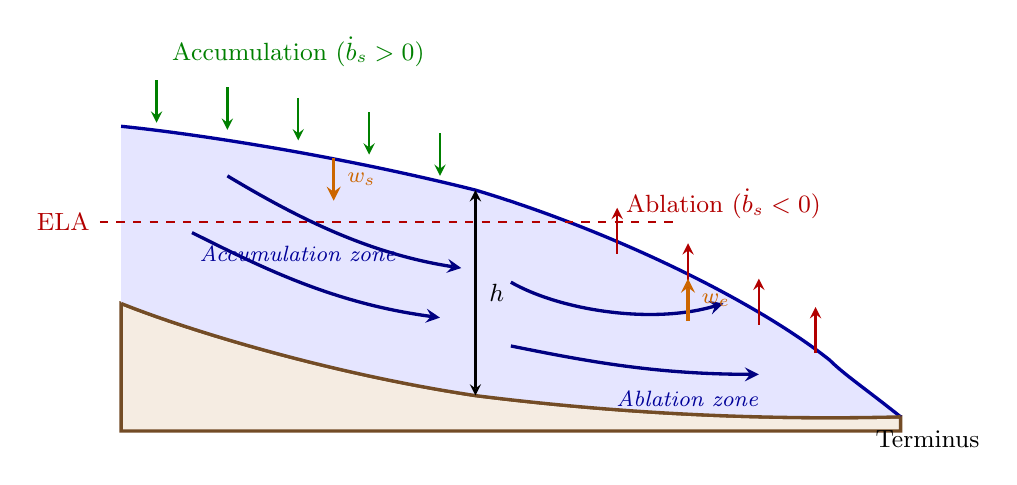
\begin{tikzpicture}[>=stealth, thick, scale=0.9]

  % Bed
  \draw[very thick, brown!60!black, fill=brown!15]
    (0,1.8) .. controls (1,1.4) and (3,0.8) .. (5,0.5)
    .. controls (7,0.25) and (9,0.15) .. (11,0.2)
    -- (11,0) -- (0,0) -- cycle;

  % Ice body (fill)
  \fill[blue!10]
    (0,1.8) .. controls (1,1.4) and (3,0.8) .. (5,0.5)
    .. controls (7,0.25) and (9,0.15) .. (11,0.2)
    -- (11,0.2)
    .. controls (10.5,0.6) and (10.2,0.8) .. (10,1.0)
    .. controls (9,1.8) and (7,2.8) .. (5,3.4)
    .. controls (3,3.9) and (1,4.2) .. (0,4.3)
    -- cycle;

  % Ice surface
  \draw[very thick, blue!60!black]
    (0,4.3) .. controls (1,4.2) and (3,3.9) .. (5,3.4)
    .. controls (7,2.8) and (9,1.8) .. (10,1.0)
    .. controls (10.2,0.8) and (10.5,0.6) .. (11,0.2);

  % Bed line (on top of fill)
  \draw[very thick, brown!60!black]
    (0,1.8) .. controls (1,1.4) and (3,0.8) .. (5,0.5)
    .. controls (7,0.25) and (9,0.15) .. (11,0.2);

  % ELA dashed line
  \draw[dashed, thick, red!70!black] (-0.3,2.95) -- (7.8,2.95);
  \node[left, red!70!black] at (-0.3,2.95) {\small ELA};

  % Accumulation arrows (snowfall)
  \foreach \xp/\ys in {0.5/4.25, 1.5/4.15, 2.5/4.0, 3.5/3.8, 4.5/3.5} {
    \draw[->, green!50!black, thick] (\xp, \ys+0.7) -- (\xp, \ys+0.1);
  }
  \node[above, green!50!black] at (2.5, 5.0) {\small Accumulation ($\dot{b}_s > 0$)};

  % Ablation arrows (melt, pointing away from surface)
  \foreach \xp/\ys in {7.0/2.55, 8.0/2.05, 9.0/1.55, 9.8/1.15} {
    \draw[->, red!70!black, thick] (\xp, \ys-0.05) -- (\xp, \ys+0.6);
  }
  \node[above, red!70!black] at (8.5, 2.85) {\small Ablation ($\dot{b}_s < 0$)};

  % Internal flow arrows (curving down in accumulation zone = submergence)
  \draw[->, blue!50!black, very thick] (1.5,3.6) .. controls (2.5,3.0) and (3.5,2.5) .. (4.8,2.3);
  \draw[->, blue!50!black, very thick] (1.0,2.8) .. controls (2.0,2.3) and (3.0,1.8) .. (4.5,1.6);

  % Internal flow arrows (curving up in ablation zone = emergence)
  \draw[->, blue!50!black, very thick] (5.5,2.1) .. controls (6.2,1.7) and (7.5,1.5) .. (8.5,1.8);
  \draw[->, blue!50!black, very thick] (5.5,1.2) .. controls (6.5,1.0) and (7.5,0.8) .. (9.0,0.8);

  % Submergence velocity annotation
  \draw[->, orange!80!black, very thick] (3.0,3.85) -- (3.0,3.25);
  \node[right, orange!80!black, font=\footnotesize] at (3.05,3.55) {$w_s$};

  % Emergence velocity annotation
  \draw[->, orange!80!black, very thick] (8.0,1.55) -- (8.0,2.15);
  \node[right, orange!80!black, font=\footnotesize] at (8.05,1.85) {$w_e$};

  % Zone labels
  \node[blue!60!black] at (2.5,2.5) {\footnotesize \textit{Accumulation zone}};
  \node[blue!60!black] at (8.0,0.45) {\footnotesize \textit{Ablation zone}};

  % Terminus label
  \node[below right] at (10.5,0.15) {\small Terminus};

  % Thickness annotation
  \draw[<->, thick] (5.0,0.5) -- (5.0,3.4);
  \node[right] at (5.05,1.95) {\small $h$};

\end{tikzpicture}
\caption{Longitudinal cross-section of a glacier showing flow trajectories, the ELA, and the submergence ($w_s$) and emergence ($w_e$) velocities.  In the accumulation zone, flow carries ice downward into the glacier; in the ablation zone, flow brings ice upward toward the surface.}
\label{fig:submergence}
\end{figure}

At any point on the glacier surface, the velocity of ice can be decomposed into a component parallel to the surface and a component perpendicular to the surface.  The perpendicular component is called the \textbf{submergence velocity} $w_s$ in the accumulation zone and the \textbf{emergence velocity} $w_e$ in the ablation zone:
\begin{itemize}
  \item \textbf{Submergence velocity} ($w_s$, accumulation zone): the rate at which ice moves downward, away from the surface.  New snow is buried and carried into the glacier interior.
  \item \textbf{Emergence velocity} ($w_e$, ablation zone): the rate at which ice moves upward, toward the surface.  Deep ice is brought up to replace mass lost by ablation.
\end{itemize}

\begin{tcolorbox}[
  colback=orange!25,
  colframe=orange!70!black,
  title={\textbf{Derivation: Submergence and Emergence Velocities from the Kinematic Boundary Condition}},
  fonttitle=\bfseries,
  breakable
]

Let the glacier surface be described by the elevation $z = s(x,t)$.  A material point on the surface moves with the ice velocity $(u_s, w_s)$, where subscript $s$ denotes evaluation at the surface.  The surface is gaining or losing mass at rate $\dot{b}_i$ (ice-equivalent thickness per unit time, measured perpendicular to the surface).  The rate of change of surface elevation must account for both:
\begin{equation}
  \frac{\partial s}{\partial t} = \dot{b}_i - u_s\frac{\partial s}{\partial x} + w_s.
  \label{eq:kinematic}
\end{equation}
The first term is the mass balance contribution; the second and third terms together give the vertical velocity of the ice surface due to ice flow.  This is the \textbf{kinematic boundary condition} at the free surface.  It follows directly from the continuity equation under the assumption that the bed is static.

\medskip
\noindent\textbf{Step 1: Define the perpendicular velocity into the ice.}  The outward unit normal to the surface is
\begin{equation*}
  \hat{\bm{n}} = \frac{1}{\sqrt{1 + \left(\partial s/\partial x\right)^2}}
    \begin{pmatrix} -\partial s/\partial x \\ 1 \end{pmatrix}.
\end{equation*}
The component of ice velocity directed into the surface (opposite to $\hat{\bm{n}}$) is
\begin{equation*}
  v_\perp = -\bm{v}_s \cdot \hat{\bm{n}}
    = \frac{u_s\,\dfrac{\partial s}{\partial x} - w_s}{\sqrt{1 + \left(\partial s/\partial x\right)^2}}.
\end{equation*}

\medskip
\noindent\textbf{Step 2: Substitute the kinematic condition.}  Rearranging \eqref{eq:kinematic} gives $u_s\,\partial s/\partial x - w_s = \dot{b}_i - \partial s/\partial t$, so
\begin{equation*}
  v_\perp = \frac{\dot{b}_i - \dfrac{\partial s}{\partial t}}{\sqrt{1 + \left(\partial s/\partial x\right)^2}}.
\end{equation*}

\medskip
\noindent\textbf{Step 3: Steady state and small surface slope.}  Taking $\partial s/\partial t = 0$ and $|\partial s/\partial x| \ll 1$:
\begin{equation*}
  \boxed{v_\perp \approx \dot{b}_i.}
\end{equation*}

\begin{itemize}
  \item In the \textbf{accumulation zone} ($\dot{b}_i > 0$): $v_\perp > 0$, meaning ice moves into the surface---this is the \textbf{submergence velocity}, $w_s = \dot{b}_i$.
  \item In the \textbf{ablation zone} ($\dot{b}_i < 0$): $v_\perp < 0$, meaning ice moves out of the surface---this is the \textbf{emergence velocity}, $w_e = -\dot{b}_i > 0$.
\end{itemize}

If the glacier is \emph{not} in steady state, the imbalance between $v_\perp$ and $\dot{b}_i$ drives the local rate of surface elevation change.  This is one way to connect surface observations (altimetry, mass balance measurements) to the underlying ice dynamics.
\end{tcolorbox}

The submergence and emergence velocities explain the characteristic shape of flow trajectories in a glacier (Fig.~\ref{fig:submergence}):
\begin{itemize}
  \item In the \textbf{accumulation zone}, flow trajectories plunge downward from the surface into the glacier interior.  Ice deposited at the surface near the head of the glacier follows a path that takes it deep into the interior before turning and flowing toward the terminus.
  \item In the \textbf{ablation zone}, trajectories curve upward toward the surface.  Ice that has traveled through the glacier interior is brought to the surface, where it is removed by ablation.
  \item At the \textbf{ELA}, flow trajectories are approximately parallel to the surface---there is neither net submergence nor emergence.
\end{itemize}

This pattern has practical consequences: ice cores drilled in the accumulation zone sample progressively older ice with depth, with the age--depth relationship controlled by the submergence velocity profile.

\subsection{Interpreting Discrepancies Between Measured and Balance Velocities}

Comparing measured velocities $U_{\text{obs}}$ with balance velocities $U_B$ diagnoses the state of the glacier:
\begin{itemize}
  \item $U_{\text{obs}} > U_B$: flux divergence exceeds accumulation $\Rightarrow$ glacier is \textbf{thinning} ($\partial h/\partial t < 0$).
  \item $U_{\text{obs}} < U_B$: accumulation exceeds flux divergence $\Rightarrow$ glacier is \textbf{thickening} ($\partial h/\partial t > 0$).
  \item $U_{\text{obs}} \approx U_B$: glacier is approximately in \textbf{steady state}.
\end{itemize}

\noindent \textbf{Examples:}
\begin{itemize}
  \item \textbf{Thwaites Glacier, West Antarctica} ($U_{\text{obs}} > U_B$ $\Rightarrow$ thinning): Measured velocities near the grounding line substantially exceed balance velocities, with flux divergence driving dynamic thinning of several meters per year.  The grounding line has retreated rapidly as ice discharge outpaces upstream accumulation---a textbook example of a glacier far from steady state (Mouginot et al., 2014; Rignot et al., 2019).

  \item \textbf{Sermeq Kujalleq (Jakobshavn Isbr\ae), Greenland} (both directions): After two decades of acceleration and thinning ($U_{\text{obs}} \gg U_B$), this glacier temporarily slowed and thickened near the terminus beginning around 2016, coinciding with a cooling of adjacent fjord waters.  The episode demonstrated the balance-velocity framework operating in reverse: reduced velocities allowed the flux divergence to decrease, and the glacier temporarily thickened ($U_{\text{obs}} < U_B$).  The glacier has since resumed acceleration (Khazendar et al., 2019).

  \item \textbf{Totten Glacier, East Antarctica} ($U_{\text{obs}} > U_B$ $\Rightarrow$ thinning): A mass-conservation (flux-gate) analysis comparing ice discharge across the grounding line with upstream surface mass balance revealed that Totten's outflow exceeds its balance flux, driving sustained thinning and grounding-line retreat.  This was significant because East Antarctica had long been considered stable; the flux-divergence approach uncovered a vulnerability that surface observations alone would not have revealed (Li et al., 2015).
\end{itemize}


\subsection{The Height--Mass Balance Feedback}

An important positive feedback arises from the coupling between glacier surface elevation and mass balance.  Consider a glacier that begins to thin in response to a climate perturbation:
\begin{enumerate}
  \item Thinning lowers the ice surface to a lower elevation.
  \item At a lower elevation, temperatures are warmer (by the atmospheric lapse rate, typically $\sim$5--7$\,^{\circ}$C\,km$^{-1}$).
  \item Warmer temperatures increase ablation and may shift precipitation from snow to rain.
  \item The more negative mass balance drives further thinning.
\end{enumerate}
This is the \textbf{height--mass balance feedback} (sometimes called the elevation--mass balance feedback).  It is a positive feedback: a perturbation that causes thinning is amplified by the resulting change in surface mass balance.

The feedback works in both directions.  A glacier that thickens raises its surface into colder air, increasing accumulation and reducing melt, which promotes further thickening.  However, this thickening branch is ultimately limited because a thicker glacier also flows faster (through the dependence of ice flux on thickness), evacuating the extra mass.

The strength of the feedback depends on the \textbf{mass balance gradient} $d\dot{b}/dz$:
\begin{itemize}
  \item \textbf{Maritime glaciers} (large $|d\dot{b}/dz|$): strong feedback, because a small change in elevation produces a large change in mass balance.
  \item \textbf{Continental/polar glaciers} (small $|d\dot{b}/dz|$): weaker feedback.
\end{itemize}

The height--mass balance feedback is the primary mechanism by which small glaciers and ice caps can undergo rapid, irreversible retreat once their surface drops below a critical elevation.

\subsection{Glacier Response Time}

How long does it take a glacier to adjust to a change in climate?  The \textbf{response time} $\tau$ characterizes the $e$-folding timescale over which a glacier approaches a new steady state following a step change in mass balance.

A useful scaling for the response time comes from comparing the volume of ice that must be added or removed to reach the new equilibrium with the rate at which mass balance can accomplish this.  For a perturbation near the terminus, the relevant scales are the ice thickness $h$ and the magnitude of the ablation rate $|\dot{b}_i|$ at the terminus:
\begin{equation}
  \tau \sim \frac{h}{|\dot{b}_i|_{\text{terminus}}}.
\end{equation}

Equivalently, the response time can be expressed in terms of the ice thickness and the mass balance gradient (J\'{o}hannesson et al., 1989):
\begin{equation}
  \tau \sim \frac{h_{\max}}{-\dot{b}_i(z_{\text{terminus}})},
\end{equation}
where $h_{\max}$ is the maximum ice thickness.  Typical values:
\begin{itemize}
  \item Small maritime glaciers: $\tau \sim 10$--50 years.
  \item Large valley glaciers: $\tau \sim 100$--300 years.
  \item Ice sheets: $\tau \sim 1{,}000$--10{,}000 years.
\end{itemize}

\noindent The response time has important implications:
\begin{itemize}
  \item Glaciers with short response times track climate changes closely and are useful climate indicators.
  \item Glaciers with long response times may still be adjusting to past climate changes---they carry a ``memory'' of earlier conditions.
  \item The height--mass balance feedback can shorten the effective response time for retreat (positive feedback accelerates the adjustment) relative to advance.
\end{itemize}

\subsection{Preview of Glacier Dynamics}

\begin{itemize}
  \item Balance velocity tells us \emph{what the velocity must be} to maintain the glacier in steady state.
  \item The mechanics (rheology, force balance, sliding laws) tell us \emph{what the velocity actually is}, given ice properties, geometry, and boundary conditions.
  \item The interplay between the two determines glacier evolution---the subject of later lectures.
\end{itemize}

%===================================================================
% SECTION 8 -- Summary
%===================================================================
\section{Summary}

Key ideas from this lecture:

\begin{enumerate}
  \item \textbf{Mass balance is the source term:} accumulation vs.\ ablation, varying with altitude, season, and climate.  It connects the glacier to the climate system.

  \item \textbf{Snow becomes ice through densification:} fresh snow transforms into glacier ice via mechanical compaction, sintering, and pore close-off.  The firn layer affects density profiles, altimetry interpretation, and meltwater storage.

  \item \textbf{Balance velocity follows from mass conservation at steady state:}
  \begin{equation*}
    U_B = \frac{1}{h\,Y} \int_{\mathcal{A}} \dot{b}_i \, d\mathcal{A}.
  \end{equation*}
  It links climate forcing directly to the velocity field without requiring knowledge of ice rheology or basal conditions.

  \item \textbf{The continuity equation} $\partial h/\partial t = \dot{b}_i - \bm{\nabla}\cdot\bm{q}$ governs how ice thickness evolves, and its surface counterpart yields the submergence and emergence velocities that control flow trajectories within the glacier.

  \item \textbf{Departures from balance} ($U_{\text{obs}}$ vs.\ $U_B$) diagnose whether a glacier is thinning or thickening---the foundation for understanding glacier response to climate change.

  \item \textbf{Feedbacks and timescales:} the height--mass balance feedback amplifies perturbations, while the glacier response time $\tau \sim h/|\dot{b}_i|_{\text{terminus}}$ sets the timescale over which glaciers adjust to climate change.
\end{enumerate}

% CHALKBOARD DRAWING 8 (leave up as summary):
% A single clean glacier side-view with:
% (a) accumulation zone and ablation zone labeled,
% (b) arrows showing flow from accumulation to ablation areas,
% (c) the ELA marked,
% (d) the balance velocity profile sketched below.
% Write the boxed balance velocity equation next to it.

%===================================================================
% Reading
%===================================================================
\section*{Reading}

Cuffey \& Paterson, \textit{Physics of Glaciers}, 4th ed.:
\begin{itemize}
  \item Sections 4.1--4.2: Mass balance overview, surface mass balance processes
  \item Sections 8.1.1--8.1.3: Ice flux, balance velocities, actual velocities
  \item Section 8.5.5: Vertically integrated continuity equations
\end{itemize}

%===================================================================
% Bibliography
%===================================================================
\begin{thebibliography}{99}

\bibitem{Adusumilli2020}
Adusumilli, S., Fricker, H.~A., Medley, B., Padman, L., \& Siegfried, M.~R.\ (2020).
Interannual variations in meltwater input to the Southern Ocean from Antarctic ice shelves.
\textit{Nature Geoscience}, 13(9), 616--620.
\texttt{doi:10.1038/s41561-020-0616-z}

\bibitem{Johannesson1989}
J\'{o}hannesson, T., Raymond, C., \& Waddington, E.\ (1989).
Time-scale for adjustment of glaciers to changes in mass balance.
\textit{Journal of Glaciology}, 35(121), 355--369.
\texttt{doi:10.3189/S002214300000928X}

\bibitem{Khazendar2019}
Khazendar, A., Fenty, I.~G., Carroll, D., Gardner, A., Lee, C.~M., Fukumori, I., Wang, O., Zhang, H., Seroussi, H., Moller, D., Noel, B.~P.~Y., van den Broeke, M.~R., Dinardo, S., \& Willis, J.\ (2019).
Interruption of two decades of Jakobshavn Isbrae acceleration and thinning as regional ocean cools.
\textit{Nature Geoscience}, 12, 277--283.
\texttt{doi:10.1038/s41561-019-0329-3}

\bibitem{Li2015}
Li, X., Rignot, E., Morlighem, M., Mouginot, J., \& Scheuchl, B.\ (2015).
Grounding line retreat of Totten Glacier, East Antarctica, 1996 to 2013.
\textit{Geophysical Research Letters}, 42(19), 8049--8056.
\texttt{doi:10.1002/2015GL065701}

\bibitem{Mouginot2014}
Mouginot, J., Rignot, E., \& Scheuchl, B.\ (2014).
Sustained increase in ice discharge from the Amundsen Sea Embayment, West Antarctica, from 1973 to 2013.
\textit{Geophysical Research Letters}, 41(5), 1576--1584.
\texttt{doi:10.1002/2013GL059069}

\bibitem{Rignot2013}
Rignot, E., Jacobs, S., Mouginot, J., \& Scheuchl, B.\ (2013).
Ice-shelf melting around Antarctica.
\textit{Science}, 341(6143), 266--270.
\texttt{doi:10.1126/science.1235798}

\bibitem{Rignot2019}
Rignot, E., Mouginot, J., Scheuchl, B., van den Broeke, M., van Wessem, M.~J., \& Morlighem, M.\ (2019).
Four decades of Antarctic Ice Sheet mass loss from 1979 to 2017.
\textit{Proceedings of the National Academy of Sciences}, 116(4), 1095--1103.
\texttt{doi:10.1073/pnas.1812883116}

\end{thebibliography}

\end{document}
